%%%%%%%%%%%%%%%%%%%%%%%%%%%%%%%%%%%%%%%%%%%%%%%%%%%%%%%%%%%%%%%%%%%%%%%%%%%%%%%%
%2345678901234567890123456789012345678901234567890123456789012345678901234567890
%        1         2         3         4         5         6         7         8

\documentclass[letterpaper, 10 pt, conference]{ieeeconf}  % Comment this line out if you need a4paper

%\documentclass[a4paper, 10pt, conference]{ieeeconf}      % Use this line for a4 paper

\IEEEoverridecommandlockouts                              % This command is only needed if 
                                                          % you want to use the \thanks command

\overrideIEEEmargins                                      % Needed to meet printer requirements.

% See the \addtolength command later in the file to balance the column lengths
% on the last page of the document

% The following packages can be found on http:\\www.ctan.org
%\usepackage{graphics} % for pdf, bitmapped graphics files
%\usepackage{epsfig} % for postscript graphics files
%\usepackage{mathptmx} % assumes new font selection scheme installed
%\usepackage{times} % assumes new font selection scheme installed
%\usepackage{amsmath} % assumes amsmath package installed
%\usepackage{amssymb}  % assumes amsmath package installed

\title{\LARGE \bf
The \textsc{TransP-0} framework for integrated transportation and power system design
}


\author{
	\IEEEauthorblockN{Dominik Ascher} \\
	\IEEEauthorblockA{
		Fakult\"at f\"ur Informatik\\
		Technische Universit\"at M\"unchen\\
		85748 Garching bei M\"unchen, Germany\\
		Email: \href{mailto:ascher@in.tum.de}{ascher@in.tum.de}
	}
	\and
	\IEEEauthorblockN{Georg Hackenberg} \\
	\IEEEauthorblockA{
		Fakult\"at f\"ur Informatik\\
		Technische Universit\"at M\"unchen\\
		85748 Garching bei M\"unchen, Germany\\
		Email: \href{mailto:hackenbe@in.tum.de}{hackenbe@in.tum.de}
	}
}


\usepackage{amsmath}
\usepackage{amssymb}
\usepackage{graphicx}
\usepackage{color}
\usepackage[colorlinks,allcolors=blue]{hyperref}
\usepackage{dblfloatfix}
\usepackage{multirow}
\usepackage{tabularx}
\usepackage{tabulary}

\newcommand{\todo}[1]{\textcolor{red}{/* #1 */}}
\newcolumntype{Y}{>{\centering\arraybackslash}X}


\begin{document}
\maketitle
\thispagestyle{empty}
\pagestyle{empty}
	\begin{abstract}
		%High penetration of electric vehicles (EV) and renewable energy sources (RES) will require fundamental changes to prevalent transportation and power systems. Intermittent and decentralized loads within the power system caused by RES and EV and the propagation of new transportation paradigms such as transportation electrification and mobility-on-demand will impose critical, closely interrelated changes on these systems.
		%Intermittent and decentralized loads caused by renewable energy sources (RES) and electric vehicles (EV) as well as 
		Increasing penetration of decentralized energy production as well as the propagation of new transportation paradigms such as transportation electrification, autonomous vehicles and mobility-on-demand will require interrelated key changes to current transportation and power systems.
		To diminish negative environmental impacts and achieve longterm sustainability, close integration between transportation and power systems is necessary and integrated planning, operation and control strategies have to be established. In this paper, we present TRANSP-0, a system design framework for rapid 
		%and iterative 
		formulation and evaluation of design options within integrated transportation and power systems. Firstly, we present the TRANSP-0 design space in terms of the static parameters for integrated subsystem design. Secondly, we visit the dynamic properties of subsystem design by formulating the underlying optimal control problem. Thirdly, we establish the requirements to integrated control strategies in terms of objectives and constraints of the described optimal control problem. Finally, we conclude with an outlook on the future scope of the proposed system design framework.
	\end{abstract}
	\section{Introduction (1.5 pages)}

% EV Motivation, Grid Impact of EVs, Balancing Demand 
In recent years, increasing awareness of environmental impacts has sparked increased interest in electric vehicles (EV) as a means to diminish dependence on fossil fuels. EVs can provide a sustainable alternative to conventional fuel vehicles if their specific demands can be sufficiently addressed by the electricty network and the transportation system.
To support the promise of a viable alternative, impacts on the power grid from EVs remain a major factor that needs to be addressed for truly smart grids, as sustainability of such a concept is strongly related with efficiently balancing energy. 
However, the efficient balancing of energy for EVs within the power grid remains a challenge - a challenge which increases with the inevitable adaption of EVs.

% Approaches for Charging Scheduling
%In recent time, approaches dealing with the optimal charging scheduling for electric vehicles have seen widespread attention in research.

Sundstrom et al. \cite{sundstrom2010planning} consider the capacity of the electricity grid in the charging of electric vehicles, thereby avoiding overloading in the grid.
Considering the necessity of charging while driving, Schlote et al. \cite{schlote2012balanced} implement load-balancing strategies for charging demand at charging points into the routing decisions of electric vehicles, resulting in reduced travel times and congestion in the traffic network. 

Furthermore, attempts to integrate intelligent charging behavior of electric vehicles into smart grids have been made. 
Alonso et al. \cite{alonso2014optimal} examine optimal charging scheduling for electric vehicles in smart grids, achieving optimal behavior for charging of EVs within a representative low-voltage net topology. The objective is oriented towards obtaining daily optimal scheduling of EV demand on transformer substations.

However, common among these approaches is that demand alleviation within the power grid represents the main objective. Therefore, differing or additional objectives as well as constraints of the traffic system, it's individual EVs and the power grid can not be represented. Furthermore, differing configurations in regard to the objectives cannot be explored and analyzed. 

% Importance of V2G + Economic impacts
Additional complexity stems from the broadness of possible interactions of EVs with the power grid. Vehicle-to-Grid (V2G) interactions are diverse in their nature and intended objectives. The economic impacts of vehicle carried batteries have been studied in the past to have significant influence ~\cite{peterson2010economics,erdinc2014economic}. Therefore, it is important to understand the specific objectives and how they influence the power grid. Furthermore, for engineering transportation systems of the future it is important to consider the constraints and objectives - for future scenarios EVs with autonomous objectives have to considered.

% Scenario definition
Examining the effects of EVs based on scenarios, Soares et al. \cite{soares2012electric} propose an electric vehicle scenario simulator, which enables the definition of electric vehicle scenarios in the context of smart grids and distribution networks. However, it's scope for scenario simulation is limited to the definition of electric vehicles scenarios and relies on external tools for specific analysis and determining impact on the power grid.

In summary, all considered approaches have in common that they aim to address the objectives of energy-efficient system behavior.

The issue remains that none of the approaches allow to rapidly explore and evaluate holistic transportation scenarios due to limited scope and intended objectives. Interfacing components of infrastructures are only partially or not considered, leading to insufficient observations about the feasibility of future transportation scenarios.

\subsection{Problem}

After studying related work, we have identified two major problems with existing approaches to future scenario modeling and exploration: First, only very basic models of the electricity network and its components are used such that a number of effects cannot be studied effectively. And second, only limited support is provided for varying the parameters of future scenarios systematically such that important variations might not be considered at all.

\subsection{Contribution}

To overcome the current situation we extend an existing approach to transportation system modeling and scenario exploration such that the electricity network can be represented in greater detail. Then we derive a systematic approach to modeling and varying the parameters of future transportation system and electricity network scenarios. Finally, we demonstrate the approach using a number of examples and discuss its strengths and weaknesses.

%The main contributions of this paper are:

%\begin{enumerate}
%	\item Description of a lightweight approach for modeling and exploring dynamics of future
%	transportation scenarios based on objectives, situations and infrastructures
%	\item Demonstration of the approach using a basic scenario employing a basic traffic network and power grid infrastructure
%	and resulting interactions with electric vehicles
%\end{enumerate}

\subsection{Outline}

In the following, we describe our approach to integrated transportation system and electricity network modeling in Section~\ref{section:contribution_1} followed by our approach to systematic parameter variation in Section~\ref{section:contribution_2}. Thereon we discuss a number of examples in Section~\ref{section:evaluation}. Finally we conclude with a summary of our contributions, remaining deficiencies and future work in Section~\ref{section:conclusion}.
	%\section{Differentiation from related work}
%\label{related_work}
%
%In the following we first review related approaches in Section~\ref{approaches} before deriving remaining issues in Section~\ref{problems}. Then, we describe the authors' background in Section~\ref{backgrounds} before summarizing the claimed contributions in Section~\ref{contributions}.

%\subsection{Related approaches}
%\label{approaches}

Intelligent \textit{scheduling} methods are widely discussed as key approaches to integrate EVs into the power grid by minimizing single or multiple objectives within power systems \cite{yang2015computational}.
% such as minimizing cost (or maximizing welfare), power losses, emissions, power deviations or optimizing battery performance of EVs within power systems \cite{yang2015computational}. 
%Here, power systems are consisted of a number of electric devices such as conventional or renewable energy sources, energy consumers as well as electric infrastructure. 
To sufficiently address technical and economic objectives, Andreotti et al.~\cite{andreotti2012review} argue for higher suitability of multi-objective optimization methods over single-objective optimization methods to evaluate model effectiveness in terms of operational limits and objective functions. 
Zakariazadeh et al.~\cite{zakariazadeh2014multi} propose a multi-objective scheduling method for EVs within a smart distribution network addressing economic and environmental objectives as well as technical constraints managing to reduce operational costs and emissions and achieve Pareto-optimal solutions.
To achieve optimal charging decisions, Ota et al.~\cite{ota2012autonomous} propose a decentralized V2G control scheme addressing the intermittency of RES energy production using electric vehicles. 
%However, the authors focus on the effects of an according charging control scheme within an isolated power system only.
%Another highly relevant direction for efficiently integrating electric vehicles into the power grid and reduce negative impacts is are approaches utilizing Vehicle Routing Problems (VRPs). Methods for vehicle routing typically focus on optimizing route selection for single or multiple traffic participants towards single or multiple objectives and a given set of constraints. Addressing objectives of energy-efficiency in terms of routing problems, Eco-Routing approaches target energy-efficient route selection. In contrast, Eco-Driving approaches target energy-efficient intermediate driving behavior ~\cite{ericsson2006optimizing}.
In contrast, Felipe et al.~\cite{felipe2014heuristic} propose multiple heuristics for \textit{routing} EVs, which consider different partial recharge strategies and technologies while traveling along routes. 
Integrating both scheduling and routing approaches, Barco et al.~\cite{barco2013optimal} present an approach for minimizing operation cost for battery EV fleets, which achieves optimal routing and charge scheduling performance.
%the approach does not consider microscopic effects on the power system when making routing and charging decisions in EVs.

%\subsection{Remaining issues}
%\label{problems}

\textit{Problems:} While the presented scheduling methods heavily address control strategies for EVs within the power system, they neglect their effects on the transportation system. In contrast, routing approaches heavily address control strategies for optimally routing single or multiple EVs within the transportation system, but do not incorporate a more detailed representation of the power system and it's underlying objectives. However, the importance of integrated planning been shown in the past for integrating electric and transportation sectors \cite{mathiesen2008integrated}. In summary, we found that current approaches do not sufficiently support control and planning of integrated transportation and power systems, i.e. formulation and evaluation of future transportation and power system design options. 

%Here, approaches often restrict the impact of electric vehicles to decisions on charging or discharging their batteries at charging stations. However, in subsequence, individual EV objectives describing routing preferences such as shortest traveling time or energy-efficiency for EVs cannot be sufficiently taken into account. Instead, emphasis is put on the power system side, while the transportation system including traffic participants isn't represented microscopically.

%VRP
%However, approaches does not take the effects of recharging within the power system into account for general cost evaluation. 
%Hence, we found that current approaches do not address sufficiently the objectives and constraints of both transportation and power systems to holistically estimate the behavior within future power and transportation system scenarios. 
%Therefore, exploring multiple objectives while planning integrated transportation and power systems remains a central issue for stakeholders. 
%To enable rapid adjustment of control strategies has to be considered, when considering rapidly changing control parameters.

%Assessing the balance of the interests of transportation systems contra the power system is a challenge, which has to be tackled in the future.

%\subsection{Claimed contributions}
%\label{contributions}
%\subsection{Authors' background}
%\label{backgrounds}

%In \cite{Hackenberg2012} we presented a model of the electric power system suitable for large-scale computation, which divides the power system into regions and subregions.
%Then, in \cite{ascher2014early} we proposed a model which represents multi-objective traffic flows as an optimal control problem and microscopically captures the mobility demands of individual vehicles within transportation systems.

%Finally, in \cite{ascher2015integrated} we presented a systems modeling technique which allows one to microscopically model and express static and dynamic interaction between components of both power systems and transportation systems.


%\subsection{Claimed contributions}
%\label{contributions}

%In this work, we describe an approach to system design for rapidly varying and evaluating parameters, objective and constraint configurations within integrated transportation and power system scenarios. 
%For this, we formally describe our model for integrated transportation and power systems in terms of the microscopic behavior of individual components. 

\textit{Contributions:} To address this situation, in this paper, we extend our previous work \cite{Hackenberg2012, ascher2014early, ascher2015integrated} and present a system design framework for rapid and iterative formulation and evaluation of design options within integrated transportation and power systems. For this we describe the underlying design space in terms of static parameters for integrated subsystem design. Then, we describe the dynamic properties of subsystem design by formulating the underlying optimal control problem. Finally, we establish the requirements to integrated control strategies in terms of objectives and constraints of the described optimal control problem.

%of the transportation and power system, i.e. individual cars and electric devices.

%Substantially, in our given model, transportation and power systems are subject to a set of different demands imposed on them. 
%Within the transportation system mobility demands are expressed by passengers, who impose (1)~position preferences including origin and destination of travel as well as (2)~time preferences, which include departure and arrival times. Currently, we restrict the considered transportation modes within our model to electric vehicles.
%Within the power system, power demands are expressed by electric devices in terms of electric power loads (or energy flows) within specific times and durations. To satisfy power demands, the power system employs power generators representing different renewable energy sources.

	%\section{Proposed approach}
\label{proposed_work}

In the following we first describe the theoretical backgrounds of our work in Section~\ref{backgrounds} before summarizing the contributions of this article in Section~\ref{contributions}

\subsection{Background}
\label{backgrounds}

%\todo{Background revisits previous work, i.e. applying software engineering techniques to smart grids, early estimation of multi-objective traffic flows, integrated transportation and power modeling}. 

% \todo{Existing, previously established systems modeling technique.}. 

%\todo{Existing, previously established model, but not sufficiently detailed}. 

%\todo{Existing, previously established technique for evaluating multiple scenarios, but focus on technique rather than results}. 

In \cite{Hackenberg2012} we presented a model of the electric power system suitable for large-scale computation. The model divides the power system into regions and subregions. In each time step for each region the power balance is calculated as the sum of all subregion power balances.

Then, in \cite{ascher2014early} we presented a model that captures the mobility demands of individual vehicles within transportation systems. For this, the technique employs a representation which formulates multi-objective traffic flows as optimal control problems. Furthermore, the transportation infrastructure is represented as directed graph, where the edges and the distances traveled on edges represent the positions of electric vehicles.

Finally, in \cite{ascher2015integrated} we presented a component-based model which allows one to express static interaction (e.g. between vehicle and controller) as well as dynamic interaction between components (e.g. vehicle and charging station). Here, the presented modeling approach allows one to microscopically model power systems based on individual electric devices and transportation systems based on individual cars in terms of components. We then proposed an integrated transportation and power system model, which allows to capture the respective demands of both transportation and power systems microscopically.

\subsection{Contributions}
\label{contributions}

In this work, we extend our previous work and formally describe our model for integrated transportation and power systems. For this, we present and detail the individual components of our model within transportation and power systems. Here, we focus on describing the microscopic behavior of individual components of the transportation and power system, i.e. individual cars and electric devices.

%\todo{Introduce scope of model in terms of demands as concept in preparation for future work.}.

Substantially, in our given model, transportation and power systems are subject to a set of different demands imposed on them. 
Within the transportation system mobility demands are expressed by passengers, who impose (1)~position preferences including origin and destination of travel as well as (2)~time preferences, which include departure and arrival times. Currently, we restrict the considered transportation modes within our model to electric vehicles.
Within the power system, power demands are expressed by electric devices in terms of electric power loads (or energy flows) within specific times and durations. To satisfy power demands, the power system employs power generators representing different renewable energy sources.

We then demonstrate our approach and employed model in a case study, where we show various scenarios for commuter traffic, which vary in terms of their traffic network structure, voltage net structure as well as employed objective weights through a number of different configurations.

%\todo{Computation: Case Study Example, varying renewable energy scenarios, different phases of renewable energy in the system}.

%\todo{Effect of EVS on indivudal systems, stabilization of power system demands}.

%\todo{Discussion of model validity? Are we there yet?}.

	\section{The \textbf{TransP-0} design space}
%\section{The \textbf{TransP-0} integrated design abstraction}
\label{proposed_model}

The \textsc{TransP-0} design abstraction is intended to support both transportation and power system engineers during early project phases in formulating and evaluating different design options quickly. Therefore, transportation and energy system properties - both static and dynamic - have to be captured sufficiently precise. On the other hand, the design abstraction should omit unnecessary details to enable frequent design iterations. With these requirements in mind we have developed a candidate design abstraction, which is summarized in Figure~\ref{system_design}. The abstraction comprises various transportation and energy subsystem parameters. Note that we have tried to reduce the number of parameters to a minimum. Hereby, we also accept potential losses in physical accuracy.

\begin{figure}[h!]
	\begin{center}
	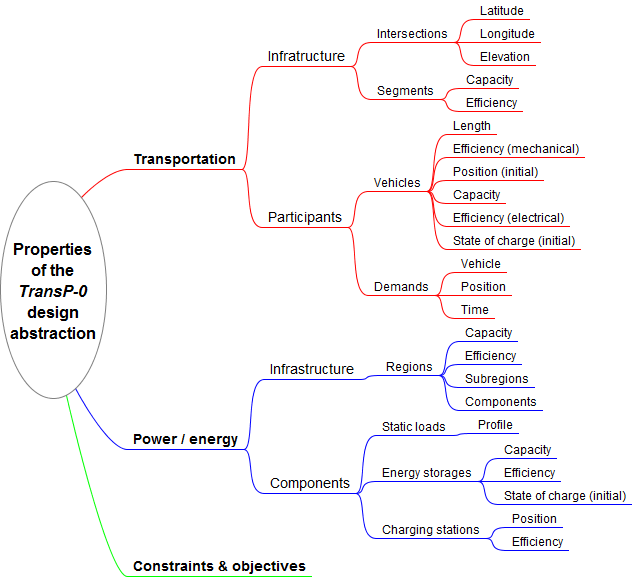
\includegraphics[trim=0 10 0 0, width=0.875\columnwidth]{./gfx/system_design.png}
	\caption{Overview over the \textsc{TransP-0} design space parameters comprising the transportation and the energy subsystem.}
	\label{system_design}
	\end{center}
\end{figure}

In the following, we first describe the design space parameters for the transportation subsystem in Section~\ref{transport} and the energy subsystem in Section~\ref{energy_system}.

\subsection{Transportation subsystem}
\label{transport}

We decided to model the transportation subsystem in a mesoscopic fashion~\cite{?}. In particular, our model includes a representation of the road network and each individual vehicle. The road network is modeled as a directed graph, where the nodes represent intersections and the edges represent the actual roads. Hereby, the edge weight defines the number of lanes and the edge direction indicates the prescribed driving direction. Consequently, two edges have to be used to describe bidirectional traffic flows. Then, the vehicles represent ''particles'' that are traveling along the road network. In particular, vehicles are assigned to points on the edges of the road network. Hence, vehicles are able to move along one edge and jump between edges at intersections. Finally, the \textsc{TransP-0} abstraction of the transportation subsystem is illustrated in Figure~\ref{transport_illustration}.

\begin{figure}[h]
	\begin{center}
	\includegraphics[trim=0 6 0 21, width=.825\columnwidth]{./gfx/transportation_system2.png}
	\caption{Illustration of a transportation subsystem design including an infrastructure (composed of road intersections and segment) and participants.}
	\label{transport_illustration}
	\end{center}
\end{figure}

Formally, the transportation subsystem $TS$ of the integrated design abstraction is modeled as a tuple $(TSI, TSP)$, where
\begin{itemize}
	\item $TSI$ represents the transportation infrastructure (i.e.\ roads and their intersections) and
	\item $TSP$ represents the individual traffic participants (i.e.\ passenger cars and goods vehicles).
\end{itemize}
Essentially, we distinguish between the static (i.e.\ the infrastructure) and the dynamic (i.e.\ the participants) parts of the transportation subsystem. In the following, we describe the the infrastructure design abstraction in Section~\ref{transport_infrastructure} before explaining the participant design abstraction in Section~\ref{participants}.

\subsubsection{Infrastructure}
\label{transport_infrastructure}

The transportation subsystem infrastructure $TSI$ of the transportation subsystem $TS$ is modeled as a tuple $(RI, RS)$, where
\begin{itemize}
	\item $RI$ represents road intersections (i.e.\ the points in geometric space where roads intersect) and
	\item $RS$ represent road segments (i.e.\ the actual roads leading from intersection to intersection).
\end{itemize}
Hence, we use a directed graph to describe the transportation subsystem infrastructure. Subsequently, we first describe the road intersections in Section~\ref{intersections} before explaining the road segments in Section~\ref{segments}.

\paragraph{Intersections}
\label{intersections}

The road intersections $RI$ of the transportation subsystem infrastructure $TSI$ are modeled - again - as a tuple $(RIL, RIC)$, where
\begin{itemize}
	\item $RIL$ represents a finite set of road intersection \textit{labels} and
	\item $RIC: RIL \rightarrow \mathbb{R}^3$ represents a mapping from road intersection labels to geometric coordinates.
\end{itemize}
Note that typically the coordinates are expressed in terms of latitude, longitude, and elevation. However, for simplicity in this work we use Cartesian coordinates instead. Consequently, distances can be computed more easily using the Euclidean metric. Moreover, transformations exist to switch between polar and Cartesian coordinates.

\paragraph{Segments}
\label{segments}

In contrast, the road segments $RS$ of the transportation subsystem infrastructure $TSI$ are modeled as a five-tuple $(RSL, RSS, RST, RSC, RSE)$, where
\begin{itemize}
	\item $RSL$ represents a finite set of road segment \textit{labels},
	\item $RSS/RST: RSL \rightarrow RIL$ represent mappings from road segment labels to their respective \textit{source} and \textit{target} road intersection labels,
	\item $RSC: RSL \rightarrow \mathbb{N}$ represents a mapping from road segment labels to their \textit{capacities} (i.e.\ the number of lanes of the road segment), and
	\item $RSE: RSL \rightarrow \mathbb{R}^+$ represents a mapping from road segment labels to their \textit{efficiency} (i.e.\ the surface material of the road segment).
\end{itemize}
Note that the previous parameters completely determine our road segment model. Consequently, we abstract from a variety of parameters typically considered such as the continuous elevation profile~\cite{?} or surface friction coefficients~\cite{?}.

Furthermore, we derive the road segment distance $RSD: RSL \rightarrow \mathbb{R}_0^+$ as a mapping from road segment labels to distances and we use the Euclidean metric $E: \mathbb{R}^3 \times \mathbb{R}^3 \rightarrow \mathbb{R}_0^+$ to compute the road segment distance as
\[
	RSD(rsl) = E(RIC(RSS(rsl)), RIC(RST(rsl))) \textrm{.}
\]
Finally, we define road segment positions $RSP \subseteq RSL \times \mathbb{R}_0^+$ as tuples of road segment labels and traveled distances
\[
	RSP = \{(rsl, d) \in RSL \times \mathbb{R}_0^+ \mid d \leq RSD(rsl)\} \textrm{.}
\]
We use the road segment positions $RSP$ to locate traffic participants (i.e.\ vehicles) on the transportation subsystem infrastructure $TSI$ as explained in Section~\ref{participants}. Note that the world coordinates can be obtained by a respective coordinate transformation.

\subsubsection{Participants}
\label{participants}

The transportation subsystem participants $TSP$ of the transportation subsystem $TS$ are modeled - again - as a tuple $(V, D)$, where
\begin{itemize}
	\item $V$ represents the vehicles (i.e.\ the physical objects using the transportation subsystem infrastructure) and
	\item $D$ represents the demands (i.e.\ the logical objects that cause the movement of the physical objects).
\end{itemize}
Consequently, we - again - distinguish between the static (i.e.\ the vehicles) and the dynamic (i.e.\ the demands) parts of the model. In the following, we first describe the vehicle design abstraction in Section~\ref{vehicles} before explaining the demand design abstraction in Section~\ref{demands}.

\paragraph{Vehicles}
\label{vehicles}

The vehicles $V$ of the transportation subsystem participants $TSP$ are modeled as seven-tuple $(VL, VS, VME, VP_0, VC, VEE, VSOC_0)$, where
\begin{itemize}
	\item $VL$ represents a finite set of vehicle \textit{labels},
	\item $VS: VL \rightarrow \mathbb{R}^+$ represents a mapping from vehicle labels to their \textit{size} (i.e.\ the length of the vehicle in road segment direction),
	\item $VME: VL \rightarrow \mathbb{R}^+$ represents a mapping from vehicle labels to their \textit{mechanical efficiency} (i.e.\ a constant ratio for the conversion between electrical and mechanical energy),
	\item $VP_0: VL \rightarrow RSP$ represents a mapping from vehicle labels to their initial road segment \textit{positions} (see Section~\ref{segments}),
	\item $VC: VL \rightarrow \mathbb{R}^+$ represents a mapping from vehicle labels to their battery \textit{capacities} (i.e.\ the maximum amount of energy that can be stored by the vehicle),
	\item $VEE: VL \rightarrow \mathbb{R}^+$ represents a mapping from vehicle labels to their \textit{electrical efficiency} (i.e.\ a constant ratio for conversion between electrical energy and stored energy), and
	\item $VSOC_0: VL \rightarrow \mathbb{R}^+$ represents a mapping from vehicle labels to their initial \textit{state of charge} (i.e.\ the amount of energy stored by the vehicle initially) such that
	\[
		\forall vl \in VL : VSOC_0(vl) \leq VC(vl) \textrm{.}
	\]
\end{itemize}
Note that again we abstract from many parameters typically considered such as the vehicle weight~\cite{?} or the vehicle geometry~\cite{?}. In particular, we approximate mechanical and electrical efficiencies with constants only.

\paragraph{Demands}
\label{demands}

Finally, the demands $D$ of the transportation subsystem participants $TSP$ are modeled as four-tuple $(DL, DV, DP, DT)$, where
\begin{itemize}
	\item $DL$ represents a finite set of demand \textit{labels},
	\item $DV: DL \rightarrow VL$ represents a mapping from demand labels to \textit{vehicle} labels (i.e.\ the concerned vehicle),
	\item $DP: DL \rightarrow RSP$ represents a mapping from demand labels to road segment \textit{positions} (i.e.\ where the concerned vehicle is expected to be), and
	\item $DT: DL \rightarrow \mathbb{N}^+$ represents a mapping from demand labels to \textit{time} points (i.e.\ when the concerned vehicle is expected to be there)
\end{itemize}
Note that our abstraction is based on discrete time. However, we do not prescribe the time step resolution. For long travel distances and durations more coarse resolutions can be used, for shorted distances and durations more fine-grained resolutions are needed typically.

\subsection{Power / energy subsystem}
\label{energy_system}

Similar to the transportation subsystem (see Section~\ref{transport}), we decided to model the energy subsystem in a mesoscopic fashion~\cite{Hackenberg2012}. Note that microscopic models represent the individual power lines and their physical characteristics~\cite{Dommel1968}, while macroscopic models aggregate the entire energy subsystem into a single market place without critical power line characteristics~\cite{Castronuovo2004}. Our mesoscopic model takes an intermediate approach, where only selected characteristics of the energy subsystem topology are represented. In particular, we limit our representation to subnetworks of equal voltage level (i.e.\ the network regions) and their hierarchical connectivity. Consequently, balances can be computed also for single regions rather than the entire electricity market. Finally, the \textsc{TransP-0} abstraction of the energy subsystem is illustrated in Figure~\ref{energy_illustration}.

\begin{figure}[h]
	\begin{center}
	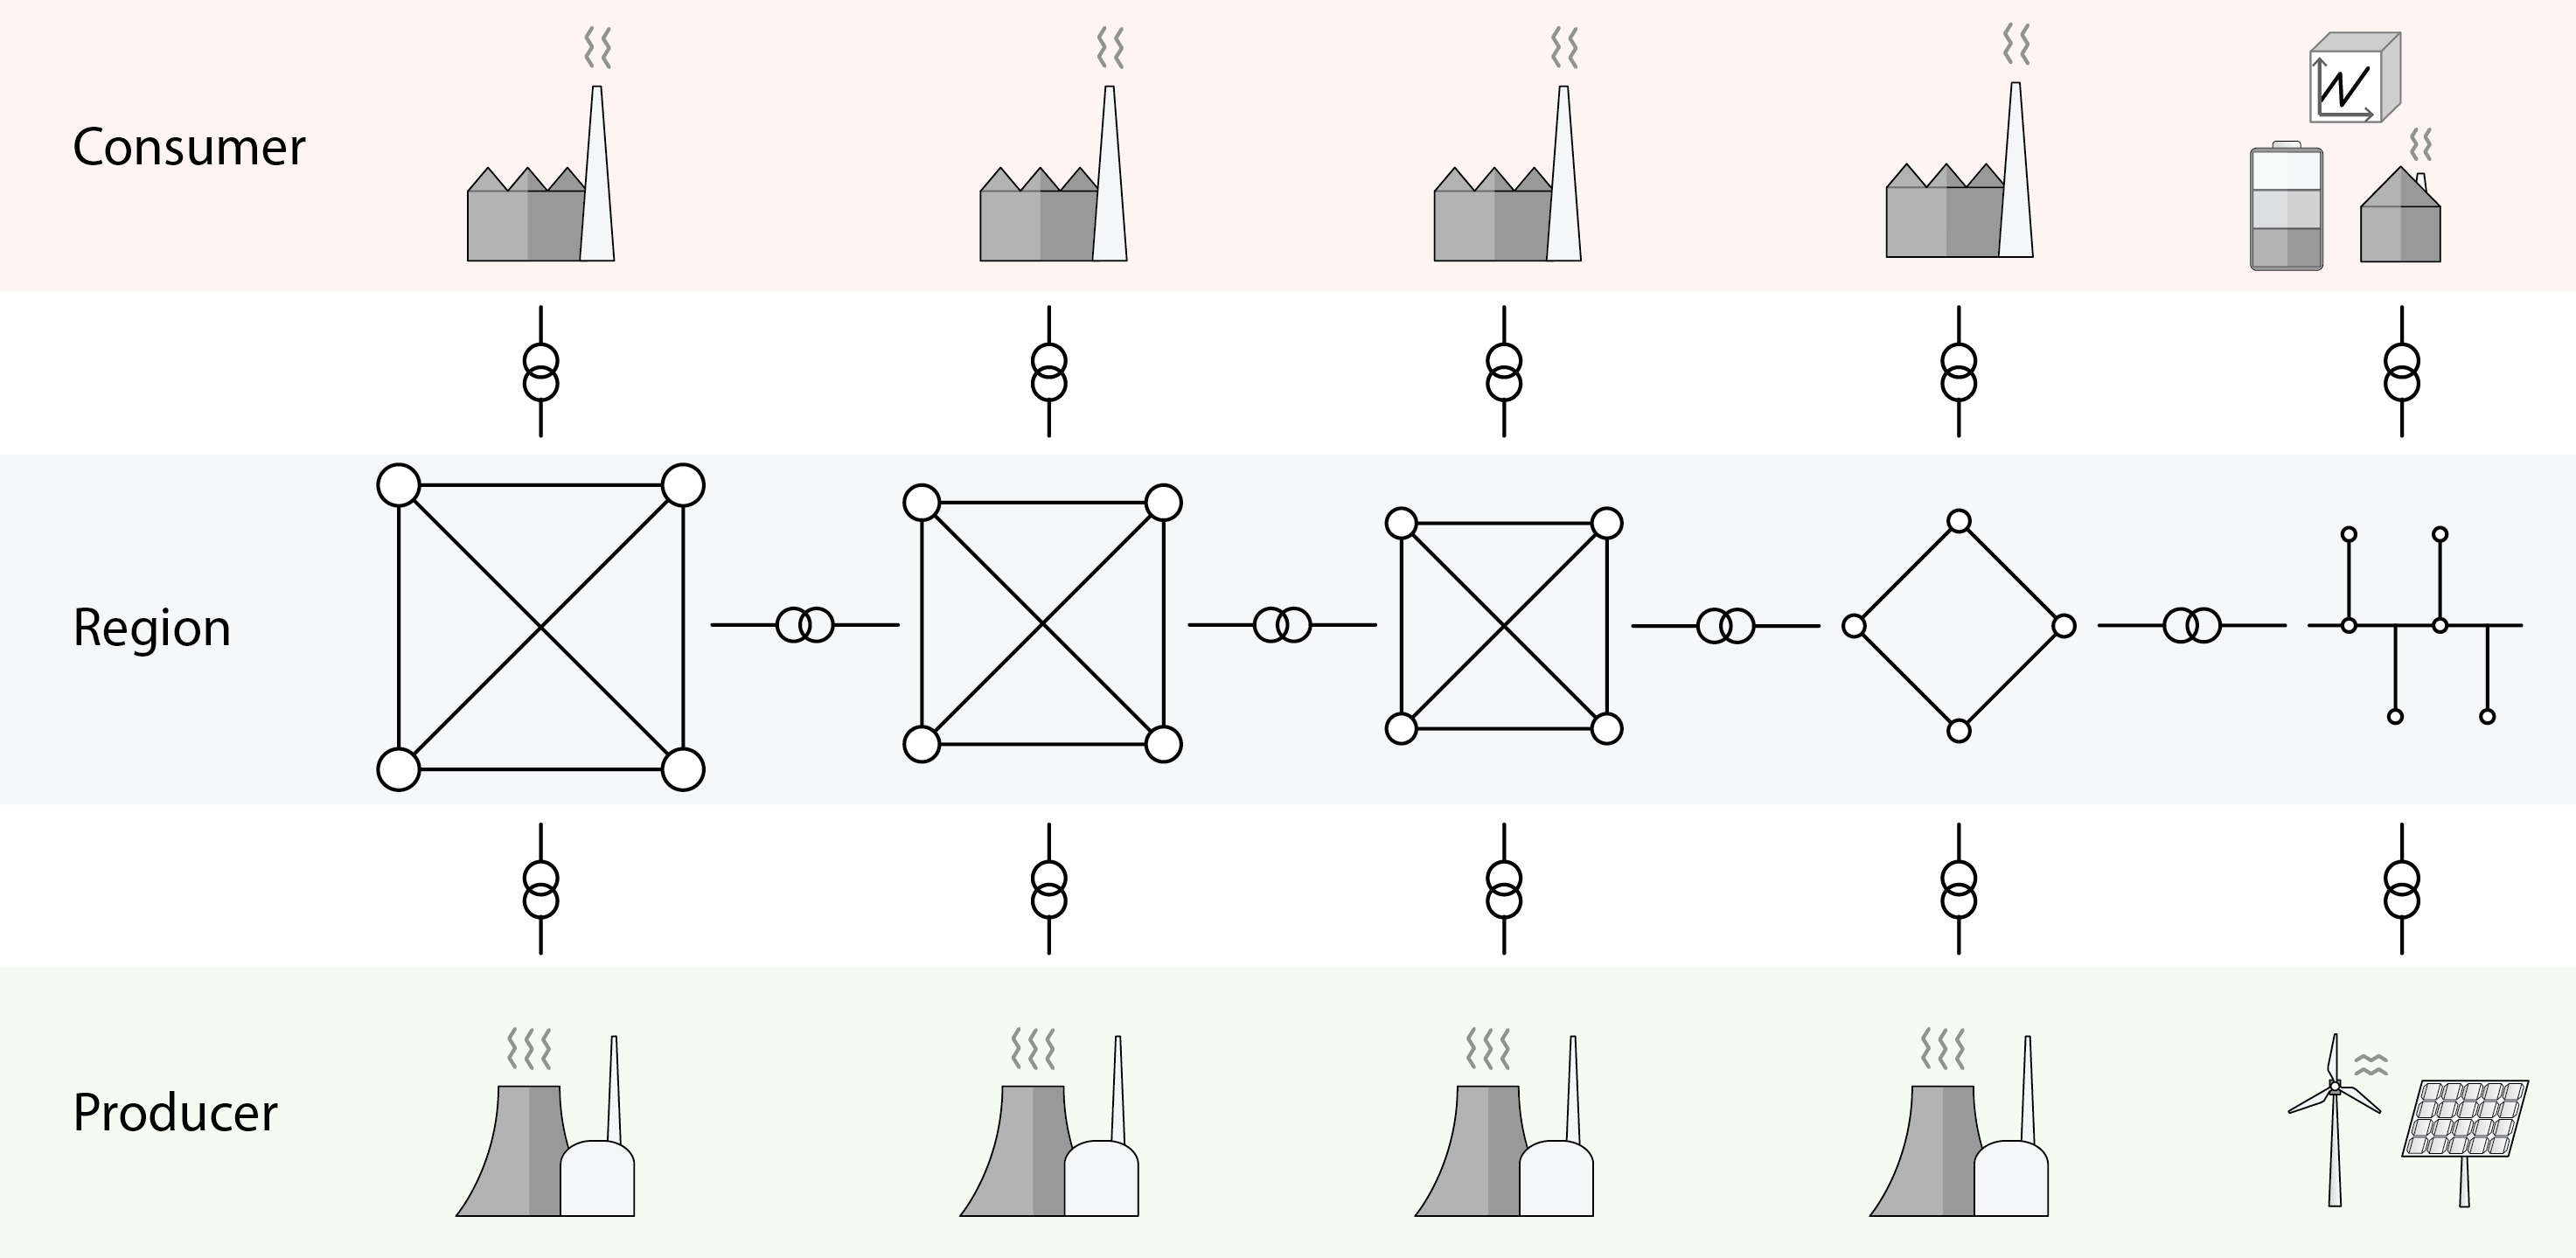
\includegraphics[trim=0 10 0 15, width=0.95\columnwidth]{./gfx/energy_system.png}
	\caption{Illustration of a energy subsystem design including an infrastructure (composed of regions) and components (i.e.\ producers and consumers).}
	\label{energy_illustration}
	\end{center}
\end{figure}

Formally, the energy subsystem $ES$ of the integrated design abstraction is modeled as a tuple $(ESI, ESC)$, where
\begin{itemize}
	\item $ESI$ represents the energy subsystem infrastructure (i.e.\ the transmission and distribution network) and
	\item $ESC$ represents energy subsystem components (i.e.\ the actual producers and consumers).
\end{itemize}
Hence, we essentially separate the network characteristics and the network usage. In the following, we first explain the infrastructure in Section~\ref{regions} before describing the components in Section~\ref{components}.

\subsubsection{Infrastructure}
\label{energy_infrastructure}

The energy subsystem infrastructure $ESI$ of the energy subsystem $ES$ is modeled as a one-tuple $(R)$, where
\begin{itemize}
	\item $R$ represents the regions of the energy subsystem infrastructure, which are determined by the voltage levels and transformers of the network.
\end{itemize}
Note that we selected a region model~\cite{Hackenberg2012} over a power flow model~\cite{Dommel1968} to reduce modeling effort and increase computational efficiency. In the following, we describe the regions in Section~\ref{regions}.

\paragraph{Regions}
\label{regions}

The network regions $R$ of the energy subsystem infrastructure $ESI$ are modeled as a four-tuple $(RL, RC, RE, RP)$, where
\begin{itemize}
	\item $RL$ represents a finite set of region labels,
	\item $RC: RL \rightarrow \mathbb{R}^+$ represents a mapping from region labels to region \textit{capacities} (i.e.\ the maximum amount of energy that can flow through that region in a predefined time interval),
	\item $RE: RL \rightarrow \mathbb{R}^+$ represents a mapping from region labels to region \textit{efficiencies} (i.e.\ a constant factor determining the energy that is lost while flowing through that region), and
	\item $RP: RL \rightarrow RP \cup \{\bot\}$ represents a mapping from region labels to their \textit{parent} region label (i.e.\ the superordinate voltage level or the start symbol $\bot$).
\end{itemize}
Note that regions must be assigned to at most one parent region. Consequently, our region model represents the energy system as a tree structure. The nodes of the tree represent \textit{subnetworks} with distinct voltage levels. The edges of the tree represent \textit{transformers} connecting the subnetworks instead. The region model can be derived easily from existing network topologies.

\subsubsection{Components}
\label{components}

The energy subsystem components $ESC$ of the energy subsystem $ES$ is modeled as a three-tuple $(SL, ES, CS)$, where
\begin{itemize}
	\item $SL$ represents the \textit{static loads} (i.e.\ loads assumed to be uncontrollable in our approach),
	\item $ES$ represents the stationary \textit{energy storages} (i.e.\ variable producers and consumers), and
	\item $CS$ represents the \textit{charging stations} for the electric vehicles (see Section~\ref{vehicles}).
\end{itemize}
In the following, we first explain the static load design abstraction in Section~\ref{static_loads}, before describing the energy storage design abstraction in Section~\ref{energy_storages} and presenting the charging station design abstraction in Section~\ref{charging_stations}.

\paragraph{Static loads}
\label{static_loads}

The static loads $SL$ of the energy subsystem components $ESC$ are modeled as three-tuple $(SLL, SLP, SLR)$, where
\begin{itemize}
	\item $SLL$ represents a finite set of static load \textit{labels},
	\item $SLP: SLL \rightarrow (\mathbb{N} \rightarrow \mathbb{R})$ represents a mapping from static load labels $SLL$ to static load \textit{profiles} (i.e.\ a predefined production and consumption curve), and
	\item $SLR: SLL \rightarrow RL$ represents a mapping from static load labels to parent \textit{region} labels (i.e.\ the region where the static load is attached).
\end{itemize}
Note that a static load profile associates a numeric load to each discrete time step. Hereby positive numbers represent energy production and negative loads represent energy consumption. Consequently, static loads can be used to model everything from home appliances to solar panels to conventional power generators. In particular, we assume such loads to be uncontrollable in our design abstraction.

\paragraph{Energy storages}
\label{energy_storages}

Then, the energy storages $ES$ of the energy subsystem components $ESC$ are modeled as a five-tuple $(ESL, ESCA, ESE, ESS_0, ESR)$, where
\begin{itemize}
	\item $ESL$ represent a finite set of energy storage \textit{labels},
	\item $ESCA: ESL \rightarrow \mathbb{R}^+$ represents a mapping from energy storage labels to energy storage \textit{capacities} (i.e.\ the maximum amount of energy that can be stored),
	\item $ESE: ESL \rightarrow \mathbb{R}^+$ represents a mapping from energy storage labels to energy storage \textit{efficiencies} (i.e.\ a constant factor between inflow energy and stored energy), and
	\item $ESS_0: ESL \rightarrow \mathbb{R}_0^+$ represents a mapping from energy storage labels to initial \textit{state of charges} (i.e.\ the amount of energy stored initially) such that
	\[
		ESS_0 \textrm{ such that } ESS_0(esl) \leq ESCA(esl) \textrm{, and}
	\]
	\item $ESR: ESL \rightarrow RL$ represents a mapping from energy storage labels to parent \textit{region} labels (i.e.\ the region where the energy storage is attached).
\end{itemize}
Note that the energy storage model is analogous to the electric vehicle model present in Section~\ref{vehicles}. However, electric vehicles additionaly define mechanical parameters, while energy storages are attached to regions statically. Furthermore, we currently target small batteries rather than large storage facilities. Larger facilities might require more parameters.

\paragraph{Charging stations}
\label{charging_stations}

Finally, the charging stations $CS$ of the energy subsystem components $ESC$ are modeled as a four-tuple $(CSL, CSP, CSE, CSR)$, where
\begin{itemize}
	\item $CSL$ represents a finite set of charging station \textit{labels},
	\item $CSE: CSL \rightarrow \mathbb{R}^+$ represents a mapping from charging station labels to charging station \textit{efficiencies} (i.e.\ a loss factor for respective energy flows), and
	\item $CSP: CSL \rightarrow RSL$ represents a mapping from charging station labels to road segment labels with zero road segment distance, i.e.\
	\[
		RSD(CSP(csl)) = 0 \textrm{, and}
	\]
	\item $CSR: CSL \rightarrow RL$ represents a mapping from charging station labels to parent \textit{region} labels (i.e.\ the region where the charging station is attached).
\end{itemize}
Note that the charging station position mapping $CSP$  and the charging station region mapping $CSR$ define the static connections between the transportation subsystem and the energy subsystem. Consequently, vehicles (see Section~\ref{vehicles}) are able to interact with arbitrary regions (see Section~\ref{regions}) of the energy subsystem infrastructure at predefined road segments (see Section~\ref{segments}).

	\section{A model of discrete-time \textbf{TransP-0} dynamics}
\label{dynamics}

While the previous section was concerned only with the static parameters of integrated transportation and energy system design, this section focuses on dynamic aspects instead. In effect, each system design defines an optimal control problem (or dynamic programming problem)~\cite{Bertsekas1995} over the transportation and energy subsystem dynamics. In the following, we describe the respective state space in Section~\ref{states}, the action space in Section~\ref{actions}, and the transition function in Section~\ref{transitions}. Note that the states, actions, and transitions do not have to be defined by the transportation and power system engineers. Rather, the definitions are the same for all system design expressed in the \textsc{TransP-0} abstraction.

\subsection{States}
\label{states}

The overall system states $S_t \in \mathbb{S}$ with time point $t \in \mathbb{N}$ of the optimal control problem are modeled as a four-tuple $(VS_t, ESS_t, CSS_t, RS_t)$, where
\begin{itemize}
	\item $VS_t$ represents the states of the \textit{vehicles} introduced in Section~\ref{vehicles},
	\item $ESS_t$ represents the states of the \textit{energy storages} introduced in Section~\ref{energy_storages},
	\item $CSS_t$ represents the states of the \textit{charging stations} introduced in Section~\ref{charging_stations}, and
	\item $RS_t$ represents the states of the \textit{regions} introduced in Section~\ref{regions}.
\end{itemize}
Note that we do not associate a state with the infrastructure of the transportation subsystem (i.e.\ we assume the infrastructure to be constant). In the following, we describe the vehicle states in Section~\ref{states_vehicles}, the energy storage states in Section~\ref{states_storages}, the charging station station states in Section~\ref{states_stations}, and the region states in Section~\ref{states_regions}.

\subsubsection{Vehicles}
\label{states_vehicles}

The vehicle states $VS_t$ of the system state $S_t$ are modeled as a tuple $(VP_t, VSOC_t)$, where
\begin{itemize}
	\item $VP_t: VL \rightarrow RSP$ represents a mapping from vehicle labels to road segment \textit{positions} (see Section~\ref{segments}) and
	\item $VSOC_t: VL \rightarrow \mathbb{R}_0^+$ represents a mapping from vehicle labels to their \textit{state of charge} (i.e. the amount of currently stored energy).
\end{itemize}
Consequently, our design abstraction neglects effects such as changing vehicle weights~\cite{?} due to passenger load or changing friction coefficients due to wheel temperatures~\cite{?}. We omitted such effects to ease design formulation primarily and replaced them with mechanical efficiency coefficients $VME$ (see Section~\ref{vehicles}), which have to be selected carefully to achieve desired statistical effects.

\subsubsection{Energy storages}
\label{states_storages}

The energy storage states $ESS_t$ of the system state $S_t$ are modeled as a one-tuple $(ESOC_t)$, where
\begin{itemize}
	\item $ESOC_t: ESL \rightarrow \mathbb{R}_0^+$ represents a mapping from energy storage labels to their current \textit{state of charge}. 
\end{itemize}
Note that we omitted advanced effects such as wear of equipment, which can cause degrading storage efficiency~\cite{?}. Again, we believe that such effects can be neglected during early phase system-level design. Furthermore, depending on the time step resolution additional state parameters are required to model - for example - ramp-up times of pumped storage hydro power plants~\cite{Garcia2008}.

\subsubsection{Charging stations}
\label{states_stations}

The charging stations states $CSS_t$ of the system state $S_t$ are modeled as a one-tuple $(CSB_t)$, where
\begin{itemize}
	\item $CSB_t: CSL \rightarrow \mathbb{R}$ represents a mapping from charging station labels to the current charging station \textit{balance} (i.e. the amount of energy sent or received from a connected vehicle).
\end{itemize}
In an advanced version of the design abstraction one could also consider failure states or software control states of charging stations. For now we assume that all charging stations work properly. Furthermore, the control strategy is provided implicitly by the optimal control problem formulation.

\subsubsection{Regions}
\label{states_regions}

The region states $R_t$ of the system state $S_t$ are modeled as a one-tuple $(RB_t)$, where
\begin{itemize}
	\item $RB_t: RL \rightarrow \mathbb{R}$ represents a mapping from region labels to the current region \textit{balance} (i.e. the aggregated loads of connected energy subsystem regions and components).
\end{itemize}
Again, we neglect physical state parameters such as power line temperatures or failure modes (e.g.\ due to exceeded temperature limits or due to environmental influences). Consequently, we assume that the energy subsystem infrastructure is available during system operation. In an advanced version of the design abstraction one might also consider failure modes and respective repair actions~\cite{?}.

\subsection{Actions}
\label{actions}

The actions $A_t \in \mathbb{A}$ with time point $t \in \mathbb{N}$ of the optimal control problem are modeled as a tuple $(VA_t, ESA_t)$, where
\begin{itemize}
	\item $VA_t$ represents the actions of the \textit{vehicles} introduced in Section~\ref{vehicles} and
	\item $ESA_t$ represents the actions of the \textit{energy storages} introduced in Section~\ref{energy_storages}.
\end{itemize}
Note that the vehicles and the energy storages are the only system components comprising actions. The states of the other components is influenced directly or indirectly by these actions. In the following, we describe the vehicle actions in Section~\ref{actions_vehicles} before explaining the energy storage actions in Section~\ref{actions_storages}.

\subsubsection{Vehicles}
\label{actions_vehicles}

The vehicle actions $VA_t$ of the system action $A_t$ are modeled as a three-tuple $(VR_t, VS_t, VB_t)$, where
\begin{itemize}
	\item $VR_t: VL \rightarrow (\mathbb{N} \rightarrow RSL)$ represents a mapping from vehicle labels to their respective \textit{route}, i.e.\ a sequence of connected road segments with $\forall vl \in VL, n \in \mathbb{N}:$
	\[
		RST(VR_t(vl)(n)) = RSS(VR_t(vl)(n + 1))
	\]
	starting at the road segment position of the previous vehicle states with $\forall vl \in VL$ and $VP_{t-1}(vl) = (rsl, d):$
	\[
		VR_t(vl)(0) = rsl \textrm{,}
	\]
	\item $VS_t: VL \rightarrow \mathbb{R}_0^+$ represents a mapping from vehicle labels to the current vehicle \textit{speed} (i.e.\ the velocity of the vehicle along the road segments), and
	\item $VB_t: VL \rightarrow \mathbb{R}$ represents a mapping from vehicle labels to vehicle \textit{balances} (i.e.\ the amount of energy sent to or received from a charging station) such that
	\[
		\forall vl \in VL: VB_t(vl) \neq 0 \textrm{ only if }
	\]
	the current vehicle speed is zero (i.e.\ the vehicle does not move) or
	\[
		 VS_t(vl) = 0 \textrm{ and }
	\]
	the vehicle is parked currently at a charging station and connected to the energy subsystem, i.e.\
	\[
		\exists csl \in CSL: VP_t(vl) = (CSP(csl), 0) \textrm{.}
	\]
\end{itemize}
Note that the routes $VR_t$ have to cover the distances traveled by each vehicle with the respective vehicle speeds $VS_t$. Hereby, the vehicle speed also can be zero such that the route only contains the previous road segment. In particular, zero speed is required to park vehicles at charging stations for one time step. Consequently, the time step resolution also determines the time intervals for charging or discharging vehicle batteries. Furthermore, note that we neglect accelerations and decelerations in the model, which might have a considerable effect on energy consumption~\cite{?}. Instead, we assume ideal conditions, which we believe to be sufficient for early phase design.

\subsubsection{Energy storages}
\label{actions_storages}

The energy storage actions $ESA_t$ of the system action $A_t$ are modeled as a one-tuple $(ESB_t)$, where
\begin{itemize}
	\item $ESB_t: ESL \rightarrow \mathbb{R}$ represents a mapping from energy storage labels to energy storage \textit{balances} (i.e.\ the amount of energy sent to or received from the parent region).
\end{itemize}
Note that physically one cannot control the (positive or negative) energy balance directly. Rather, for a pumped storage hydro power plant one might control a valve limiting the downhill water flow and an electric drive causing the uphill water flow~\cite{Castronuovo2004}. In fact, the actual control parameters depend on the concrete storage type. We believe that considering the energy balance directly represents the smallest common denominator.

\subsection{Transition function}
\label{transitions}

The transition function is a mapping
$
	T: \mathbb{S} \times \mathbb{A} \rightarrow \mathbb{S}
$ describing the transition from a state, given an action to a new state.
Stepping forward in time, the transition function is then defined as a function
\[
	T(S_t, A_t) = S_{t+1} \mathrm{,}
\]
where $S_{t+1}$ describes the state following $S_t$ after choosing action $A_t$. Accordingly, the transition function $T$ is then

The individual vehicle state
\begin{itemize}
	\item $VS_{t+1} = f(VS_t, VA_t)$ represents ...,
	\item $ESS_{t+1} = g(ESS_t, ESA_t)$ represents ...,
	\item $CSS_{t+1} = h(VS_{t+1}, VA_t)$ represents ..., and
	\item $RS_{t+1} = i(CSS_{t+1}, ESA_t)$ represents ....
\end{itemize}
\todo{Outline.}

\subsubsection{Vehicles}
\label{transitions_vehicles}

\todo{Introduction.}
\begin{itemize}
	\item $VP_{t+1} = f_1(VP_t, VR_t, VS_t)$ represent ... and
	\item $VSOC_{t+1} = f_2(VP_t, VSOC_t, VR_t, VS_t, VB_t)$ represents ....
\end{itemize}
\todo{Wrap-up.}

\subsubsection{Energy storages}
\label{transitions_storages}

\todo{Formalize!}

\subsubsection{Charging stations}
\label{transitions_stations}

\todo{Formalize!}

\subsubsection{Regions}
\label{transitions_regions}

\todo{Formalize!}
	
\section{Objectives and Constraints}
\subsection{Constraints}
\label{constraints}

In principle, one can define arbitrary constraints over the static and dynamic system properties presented in the previous sections. In particular, we believe that such constraints might arise from design decisions made by transportation and energy system engineers. Hence, we do not want to prescribe the constraints. Rather, we provide two basic constraints which we believe to be part of any integrated system design. The first constraint makes sure that the road segment capacities $RSC$ (i.e.\ the number of lanes) of the transportation subsystem infrastructure $TSI$ are not exceeded (see Section~\ref{collisions}). The second constraint makes sure that the region capacities $RC$ of the energy subsystem infrastructure $ESI$ are not exceeded (see Section~\ref{capacities}).

\subsubsection{Segment capacities}
\label{collisions}

TODO

%Overlapping vehicle pairs $OVP : \mathbb{VS} \rightarrow V \times V$
%\[
%OVP(VS) = \{(v_1, v_2) \in V \times V \mid
%\]
%\[
%((rs_1,rd_1),\cdot) \in VS(v_1), ((rs_2,rd_2),\cdot) \in VS(v_2) :
%\]
%\[
%rs_1 = rs_2 \wedge (|rd_1 - rd_2| < VL(v_1) / 2
%\]
%\[
%\vee
%\]
%\[
%|rd_1 - rd_2| < VL(v_2) / 2)\}
%\]
%Overlapping vehicle sets $OVS : \mathbb{VS} \times V \rightarrow \mathcal{P}(V)$
%\[
%OVS(VS,v) = \{v' \in V \mid (v, v') \in OVP(VS)\}
%\]
%Collision property $CV : \mathbb{VS} \rightarrow \mathbb{B}$
%\[
%CV(VS) \Leftrightarrow \exists v \in V :
%\]
%\[
%|OVS(VS, v)| > RSL(rs) \text{ with } ((rs,\cdot),\cdot) = VS(v)
%\]

\subsubsection{Region capacities}
\label{capacities}

TODO

\subsection{Objectives}
\label{objectives}

In addition to constraints (see Section~\ref{constraints}), our approach supports arbitrary objectives over the static and dynamic properties of the transportation system (see Section~\ref{transport}) and the energy system (see Section~\ref{energy_system}). In particular, we do not want to prescribe any particular objectives. Rather, we believe that it is the designers task to formulate different objectives and explore their effect on the system structure and dynamics. 
%For demonstration (see Section~\ref{demonstration}) we selected objective that we have used also in previous work. 
Among objectives we consider minimizing traveling times, minimizing energy consumption during driving, and minimizing the energy disbalance of the energy subsystem. Other objectives might include for example minimizing the free road segment space or minimizing energy storage usage.
	%\section{Using the \textbf{TransP-0} design abstraction}
\label{demonstration}

In the following, we evaluate \textsc{TransP-0}. Therefore, we first present prototypical tool support in Section~\ref{tool}, which we have used for coding the actual system designs and optimizing their behavior. Then, we describe the sample system design in Section~\ref{examples}, which are intended to show the capabilities of the design abstraction. Finally, we discuss the results of and experiences made during the experiments in Section~\ref{discussion}. In particular, we are interested in the suitability of the design abstraction with respect to rapid and iterative design formulation as well as evaluation.

\subsection{Prototypical tool support}
\label{tool}

TODO

\begin{figure}[h]
	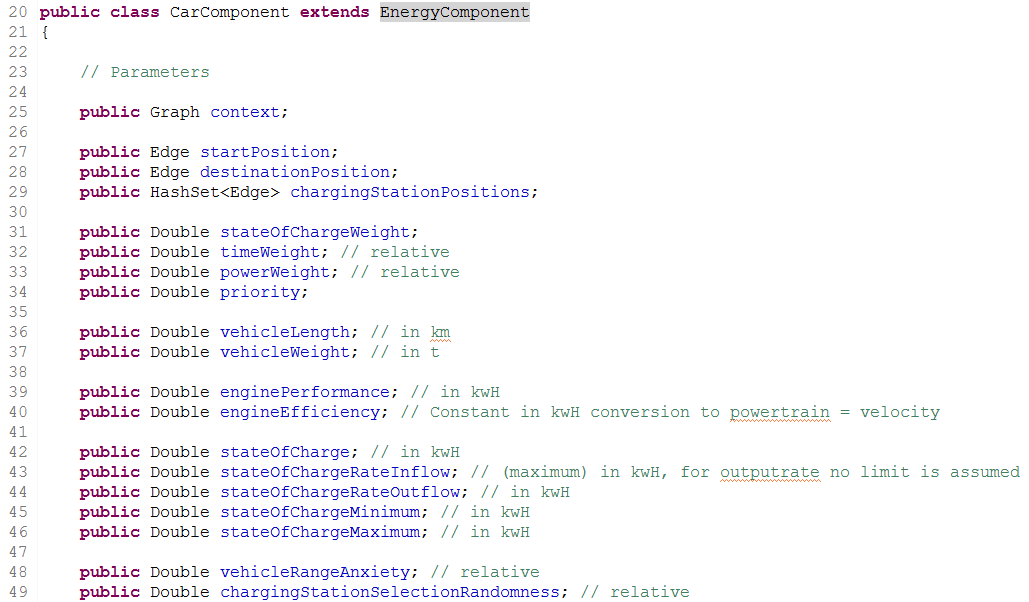
\includegraphics[width=\columnwidth]{./gfx/modeling.png}
	\caption{System modeling using regular Java classes and the Eclipse integrated development environment (IDE).}
	\label{figure:modeling}
\end{figure}

TODO

\begin{figure}[h]
	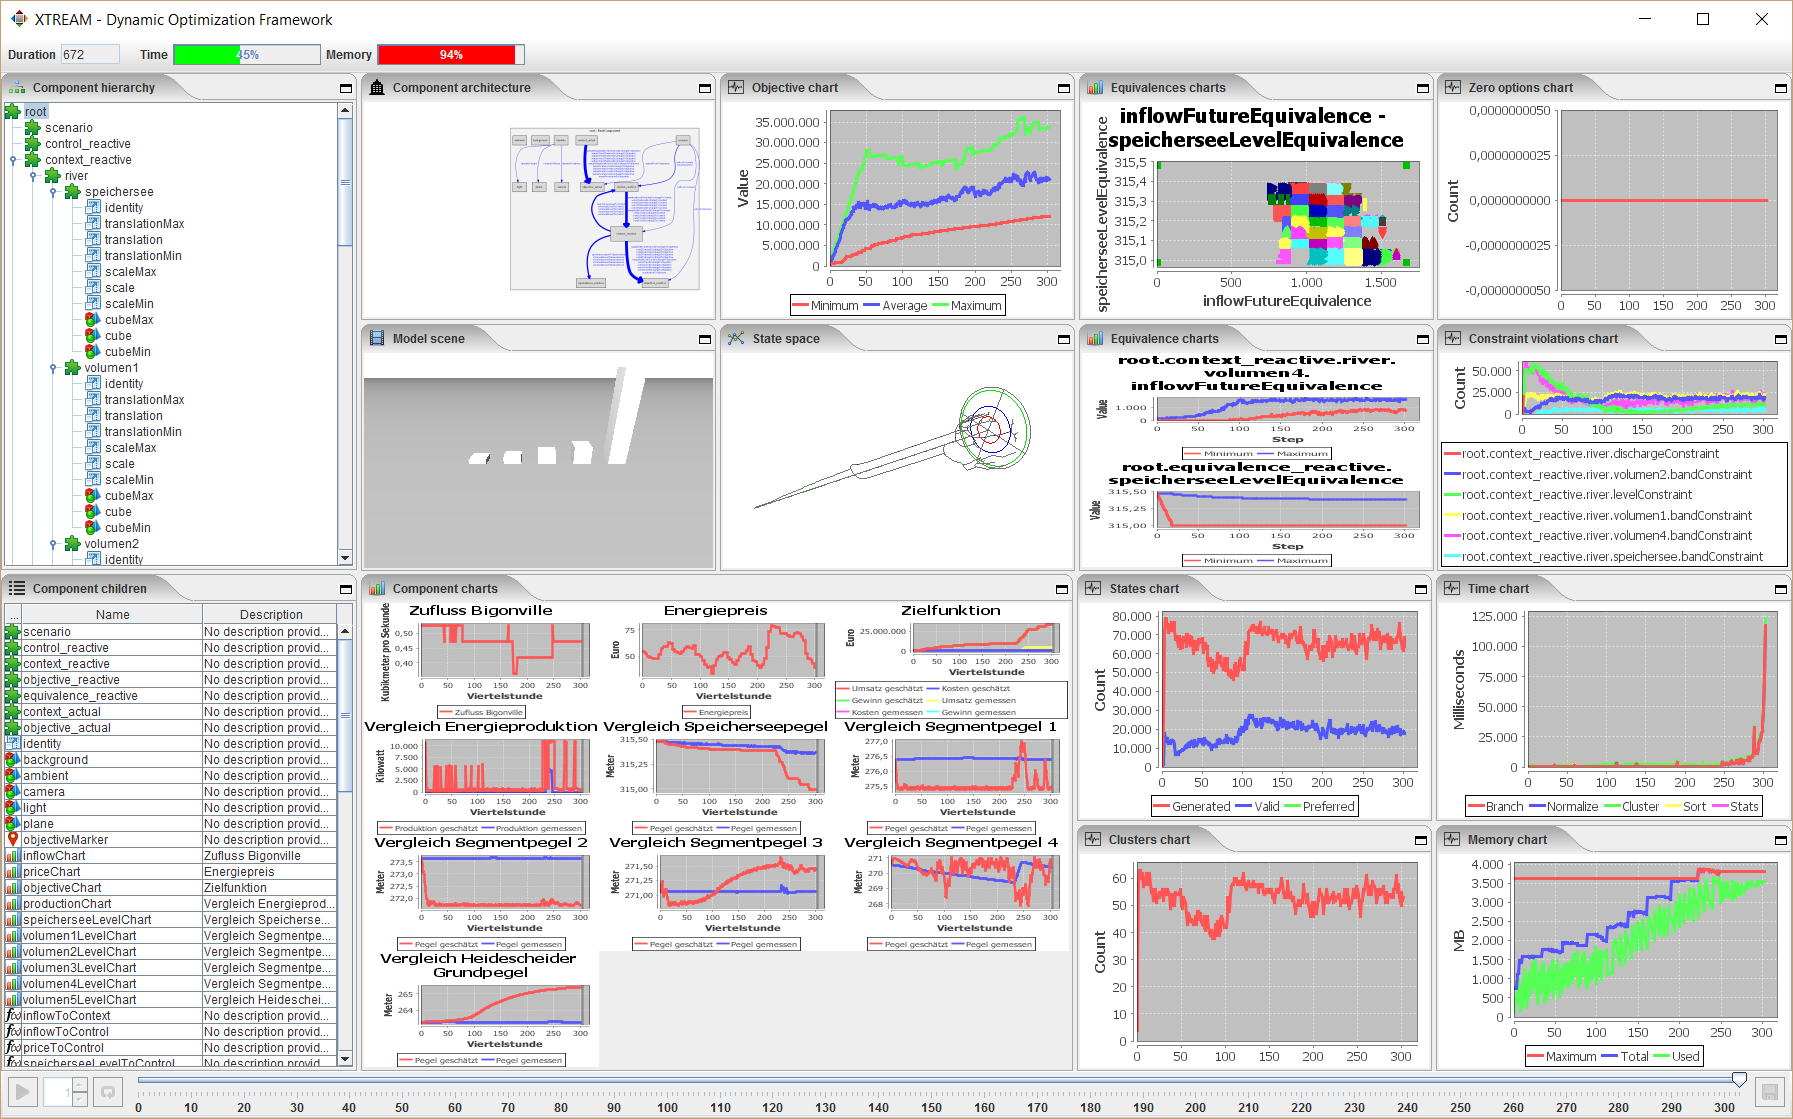
\includegraphics[width=\columnwidth]{./gfx/analysis.png}
	\caption{Model analysis using a basic approximate dynamic programming algorithm and comprehensive visualization techniques.}
	\label{figure:analysis}
\end{figure}

TODO

\subsection{Exemplary system designs}
\label{examples}

In this case study we propose a simple scenario for commuter traffic where ten traffic participants travel from home to work locations. In each time step traffic participants actions consist in selecting driving speed, time of charging, time of departure as well as route selection when driving towards their respective destination positions. The selected traffic infrastructure is consisted of a traffic network of 20 by 5 kilometers with two possible origins and two possible destinations of travel for individual traffic participants. 

\begin{figure}
	\centering
	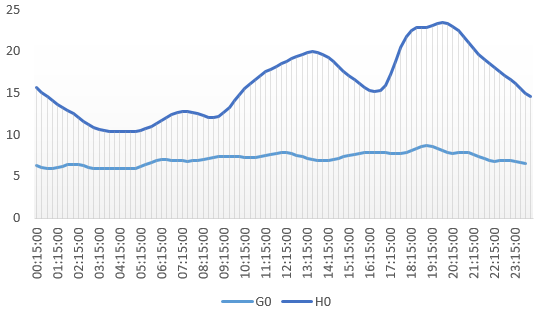
\includegraphics[width=\columnwidth]{gfx/profiles.PNG}
	\caption{Illustration of home (H0) and workplace (G0) load profiles.}
	\label{profiles}
\end{figure}

Subsequently, we evaluate traffic scenarios in terms of different configurations varying in their respective parameters. 

\subsubsection{Configuration 1: Objective function structure}

We consider three different scenarios when varying objective weight configuration: (1) focus on achieving energy-efficiency with regard to driving and power system balance, (2) focus on achieving shortest traveling time while driving as well as (3) an intermediate configuration of both energy-efficiency and shortest traveling time.

\subsubsection{Configuration 2: Voltage net structure}

We consider a changing voltage net structure within two configurations: (1) single voltage nets aggregating both the consumers and producers of home and workplaces as well as (2) allocation of two distinct voltage nets for the consumers and producers of home and workplaces. 

\subsubsection{Configuration 3: Traffic network structure}

Finally, we evaluate scenarios with regard to variation of the structure of the employed traffic network. Here, we vary the number of possible paths for traffic participants to travel from home to workplace destinations and vice versa.  

The results are pictured in Figure \ref{figure:examples}. 

\begin{table*}[b]
	\centering
	\renewcommand{\arraystretch}{1.3}
	\begin{tabularx}{\textwidth}{|Y|Y|Y|Y|}
		\hline
		
		\textbf{Scenario 1} & \textbf{Scenario 2} & \textbf{Scenario 3} \\
		
		\hline
		
		Energy-efficiency &
		Shortest traveling time &
		Intermediate \\
		
		\hline
		
		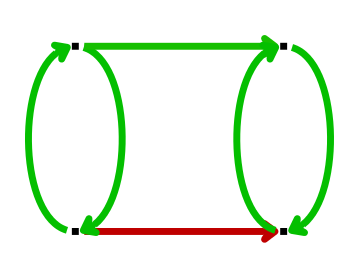
\includegraphics[width=0.20\textwidth, trim=0 0 0 -3]{gfx/Graph2.png} &
		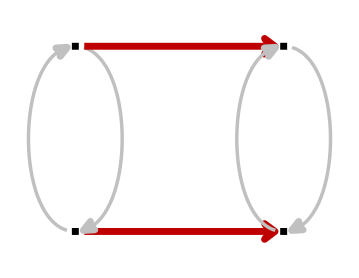
\includegraphics[width=0.20\textwidth, trim=0 0 0 -3]{gfx/Graph1.png} &
		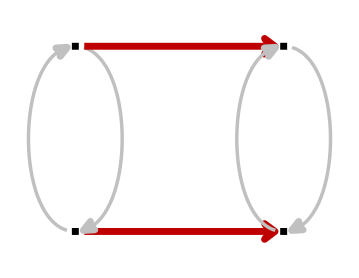
\includegraphics[width=0.20\textwidth, trim=0 0 0 -3]{gfx/Graph1.png} \\
		
		\hline
		
		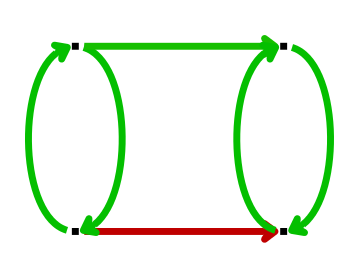
\includegraphics[width=0.20\textwidth, trim=0 0 0 -3]{gfx/Graph2.png} &
		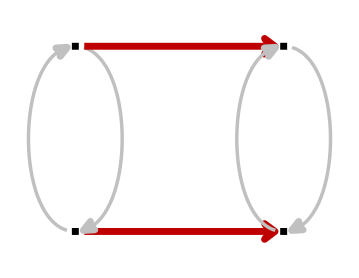
\includegraphics[width=0.20\textwidth, trim=0 0 0 -3]{gfx/Graph1.png} &
		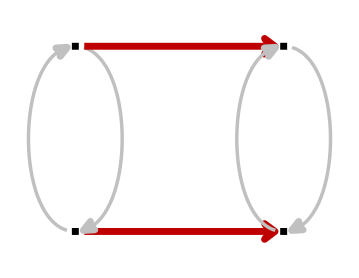
\includegraphics[width=0.20\textwidth, trim=0 0 0 -3]{gfx/Graph1.png} \\
		\hline			
	\end{tabularx}
	\caption{Traffic flow graph and power charts for different configurations.}
	\label{figure:examples}
\end{table*}
	%\section{Discussion}
\label{section:discussion}

In the following we discuss our approach with respect to four questions: How \textit{valid} are the underlying system models and the behavior estimation results? How \textit{novel} is the approach compared to existing studies on electro-mobility? How \textit{efficient} is the technique to evaluate different scenarios? And finally how \textit{applicable} is our approach in practice?

\subsection{Validity}

The scope of our approach is to provide an overview of possible behavior during early phases of systems engineering. In this context, for system modeling we employ high-level models, which provide an estimation of system behavior. Therefore, it has to be shown whether according behavior specification and estimation prove to be valid compared with detailed traffic and electrical network simulations. In presented examples, model state is evaluated in steps of 60 seconds over all total time of 30 minutes, showing only a small portion of behavior over time. However, computational complexity of models during behavior optimization could represent an issue, as continuous values of time and state have to be considered. In contrast, in our model, values of state and time are modeled in discrete steps to reduce computational complexity.

The proposed approach provides an estimation over traffic and energy flows within high-level scenarios. In terms of the traffic infrastructure, a representation of the traffic network has been employed, on which behavior of individual cars can be observed microscopically. Currently, a traffic network of 45km in width and 45km in length is considered. More detailed traffic networks could be employed to more accurately represent real world traffic infrastructures. Our current traffic network neglects low-level infrastructure such as traffic lights and turns within roads. Furthermore, the currently employed vehicle model doesn't consider acceleration, deceleration and gravitational forces during turns, but uses average values for speed and energy consumption instead. Centrally, it also remains an issue, whether the parameters employed in our scenarios are representative for real-world scenarios.

In terms of the power system and electric infrastructure, only a basic net architecture consisting of two levels, i.e. low and medium voltage nets, is considered, neglecting a representative structure found in real world circumstances. Further abstraction is employed by static profile components, which aggregate intermittent net loads over time, representing high-level abstractions with diminished accuracy. Furthermore, charging 
and discharging of cars at charging stations utilizes static loads in contrast to variable loads, due to reduction of possible behavior space and computational complexity. In Summary, comparison between our approach and implementation in a simulation framework like SUMO could provide a means for validation of our approach, especially in terms of behavior the transportation system.

%In the results obtained from the examples, it has been shown that total load balance equalization was achieved to a higher degree, when the weight of the power system cost function was higher. In contrast, when more weight was put on the transportation system cost function, findings showed total load balance equalization to a lower degree. 
It remains an issue, whether such an objective distinction between different systems and according objective parameter variation can be applied to real world scenarios when considering a very high number of potentially involved objectives. Furthermore, to reduce complexity, several objectives of EVs which are of main interest to drivers such as battery degradation and energy price have been neglected in our model, but are important issues of the V2G concept which have to be addressed in the future.

\subsection{Novelty}

We employ a parameter-based approach allowing for rapid modeling and evaluation of multi-objective transportation and power system scenarios. Compared to existing approaches outlined in Sec.~\ref{section:retrospection}, model formulation and adjustment can be rapidly achieved in terms of individual composition of involved systems, independently of underlying objectives. Fundamentally, our approach allows one to concisely assess situations within transportation and power systems. As demonstrated in Sec.~\ref{section:evaluation}, this enables one to rapidly evaluate novel scenarios concerning different systems, e.g. different expansion levels of renewable and smart energy penetration. 

\subsection{Efficiency}

At its core, our approach represents a rapid prototyping technique, enabling to formulate, estimate and evaluate scenarios concerning multiple systems. For this, we employ incremental techniques which allow model refinement through multiple iterations. Here, the efficiency of our approach can be measured in terms of lines of code (LOC) necessary to establish a given scenario. Avoiding time and resource intensive modeling, our approach has shown to allow quickly establishing medium complexity scenarios within 350 LOC. However, multiple iterations when establishing scenarios have to be factored in, as LOC do not represent an accurate measure for effort, but rather for ease of modeling.

\subsection{Applicability}

In terms of planning transportation and power systems, for our approach it remains an issue of applicability allowing to rapidly evaluate scenarios. The applicability of the approach is strongly dependent on involved domain knowledge, providing insight into involved systems. However, a major issue represents the fragmentation into different domains and involved goals with transportation systems being regulated by government bodies and electric networks being regulated by private entities. Therefore, practical applicability of transportation and power system modeling and evaluation depends on separated domains collaborating.
	\section{Conclusion}
\label{section:conclusion}

In this paper, we proposed an approach to rapidly model and evaluate transportation and power system scenarios. 
%For this, we extended an existing approach to transportation system modeling and scenario exploration to include a suitable representation of the power system. 
The proposed holistic and component-based approach is able to model power systems with detailed electric devices as well as transportation systems with individual cars microscopically. Our approach allows to rapidly explore and vary configurations of transportation system and electric network scenarios. We evaluated several incremental scenarios varying in stage of expansion of renewable and smart energy devices as well as focus of system objectives. 
%the weight of objectives of transportation and power systems. 
Scenario results demonstrated the feasibility of the modeling technique and rapid evaluation of multiple scenarios. However, key issues which have to be addressed are the validity and applicability the approach.
Future work includes refinement of model accuracy through vehicle model improvements and utilization as well as modeling of additional objectives and systems. Furthermore, modeling representative traffic infrastructures with OpenStreetMap and validation of results obtained with our approach represent major next steps. Finally, to be able to handle larger problem scales, more detailed models and resulting computational complexity, we currently work on effective behavior estimation algorithms.

	
	\bibliographystyle{bst/IEEEtran}
	\bibliography{references}




\end{document}
